The GDELT data subset we use in this project consists of sixty
three thousand csv files, where each file takes somewhere between
800 KB and 1.5 MB of storage.

On our P2 hand-in we include a script
(/gdelt/download.py) that downloads each csv file
and edits the filenames for further processing.
If a file is found to be corrupt, it is not downloaded and
the index of the file is saved in a .txt file
(/gdelt/bad\_indices.txt).

The dataset consists of sixty attributes and the domain of
each attribute is in detail on the official handbook
{\color{red}{citation}}.
\cite{suicide_website}

Moving on, the suicide rate dataset can be obtained by
navigating to the Centers for Disease Control and Prevention
website

\begin{figure}
	\centering
	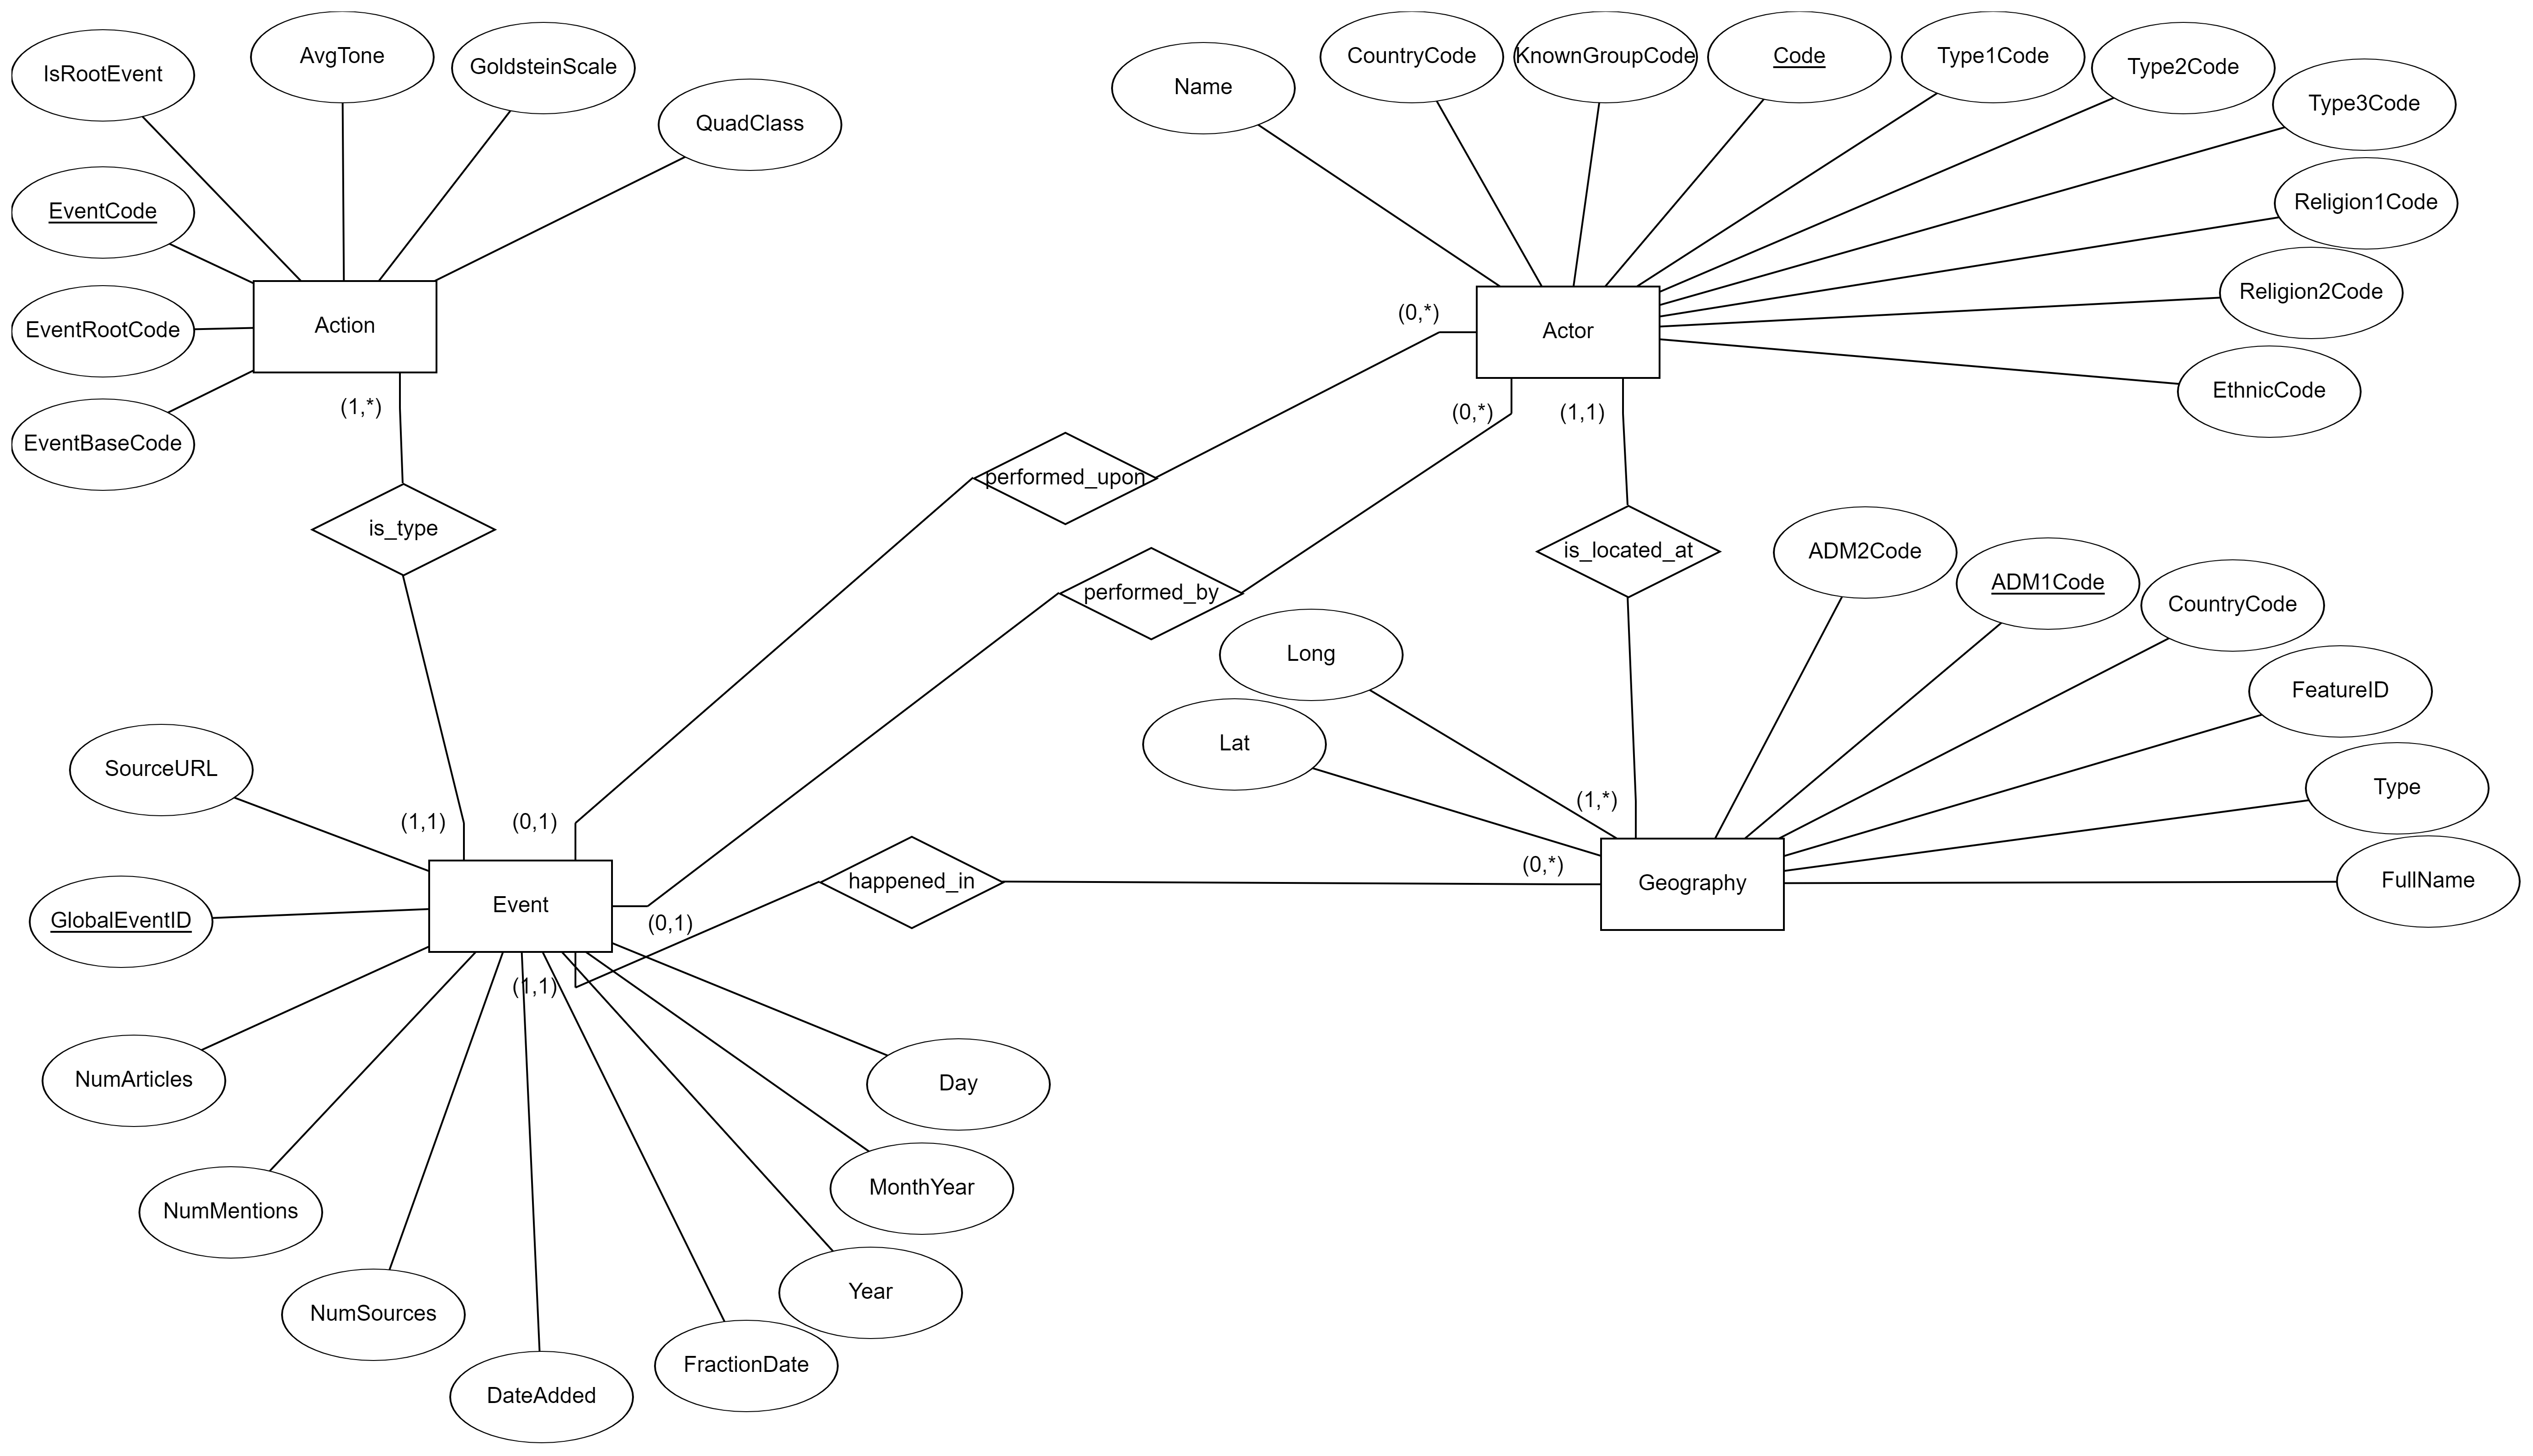
\includegraphics[scale = 0.08]{gdelt.png}
	\caption{Our GDELT schema integration}
	\label{fig:gdelt}
\end{figure}
